\documentclass[12pt,a4paper]{report}
\usepackage[utf8]{inputenc}
\usepackage{amsmath}
\usepackage{amsfonts}
\usepackage{amssymb}
\usepackage{graphicx}

\input defs.tex
\bibliographystyle{alpha}
\graphicspath{ {./figures/} }



\title{Neural Network Based Decoding over Molecular Communication Channels}
\author{Peter Hartig}

\begin{document}
\maketitle

\begin{abstract}

\end{abstract}

\newpage
\tableofcontents
\newpage

\section{Introduction}
Characterizing and obtaining information about communication channels is a fundamental barrier to communication. While optimal and sub-optimal strategies for overcoming this barrier in many contexts have enabled vast and effective communication infrastructure, this barrier still limits communication in others. Molecular Communication channels pose a particularly difficult context in which to overcome this barrier as channel characteristics are often non-linear and may be dependent on the specific transmitted information stream.
In communication contexts, such as wireless, long, "Pilot" symbol-streams are often used to mitigate the difficultly in obtaining channel information by provide real-time information supporting an underlying channel model. The low symbol rate of Molecular Communication channels often makes such strategies impractical. However, the success of this data-driven technique in wireless channels suggest that perhaps an alternative, data-driven method may be viable in the Molecular Communication context. One potential data-driven method for characterizing these channels is a neural network. Neural networks have shown to be an effective tool in data-driven approximating of probability distributions.
\par

The general communication channel is equivalent to a conditional probability $P(x|y)$, in which $x$ is transmitted information and $y$ is received information.  $P(x|y)$ takes into account the (potentially random) channel through which the information $x$ passes, and random noise added prior to receiving $y$. The communication problem entails optimizing a form of $P(x|y)$ over a set of possible, transmitted information. In general, sub-optimal solutions do not require perfect knowledge of the distribution $P(x|y)$ and may be used when $P(x|y)$ is unknown or impractical to obtain. In this work, a neural network is used to estimate $P(x|y)$.

\section{System Model}

\subsection{MLSE}


\section{Numerical Results}
\subsection*{ViterbiNet}
	\includegraphics[width=\textwidth,height = 7cm]{lti_standard}
	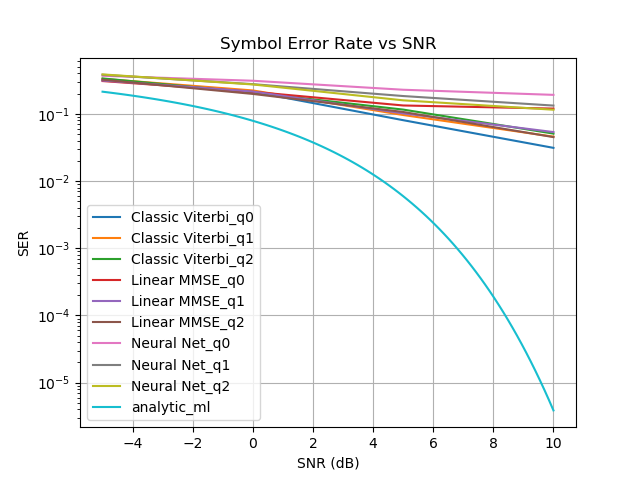
\includegraphics[width=\textwidth,height = 7cm]{quant_standard}

\subsection*{Reduced State ViterbiNet}
	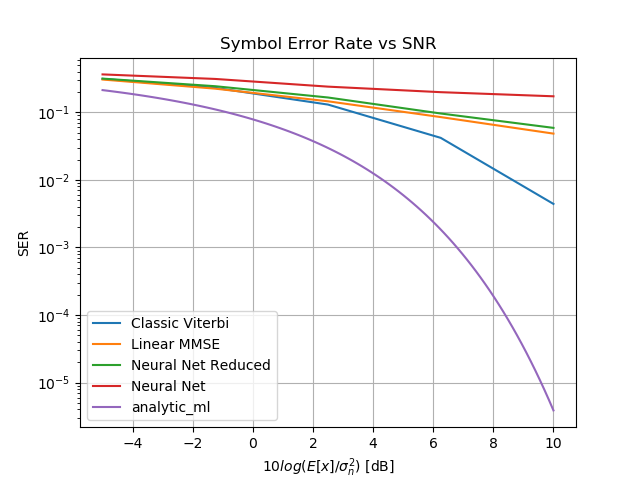
\includegraphics[width=\textwidth,height = 7cm]{lti_reduced}
	\includegraphics[width=\textwidth,height = 7cm]{quant_reduced}
\section{Conclusion}

\newpage
\bibliography{mc_report}
\end{document}